
\section{\NAME{}}
\label{sec:proposal}

\NAME{} (polyLogarithmic SEQuence) is the name of the proposed allocation
function. As such, any sequence data structure using variable-size identifiers
can use it. \NAME{} allocates identifiers with a space complexity
polylogarithmically upper-bounded with respect to the number of insert
operations. Since sequence data structures scale in the number of peers and the
concurrency rate, building a distributed collaborative editor using \NAME{}
would allow ergonomic and massive collaborative editing of huge documents. This
section describes \NAME{}: $allocPath$ and $allocDis$ functions. Then, it
provides the proof of the space complexity of its identifiers.

\begin{asparadesc}
\item [The function allocPath] chooses the path associated with each element in
  order to encode its relative position with regard to its adjacent elements in
  the sequence. For the sake of performance, the aim of $allocPath$ is to keep
  the underlying tree with a small depth. Three components compose
  $allocPath$. Each of these components fails to provide an efficient
  allocation function. Nevertheless, their composition allows to get the best
  of each by cancelling their respective deficiency.
\end{asparadesc}

\begin{enumerate}[leftmargin=*]
\item The first component is an exponential
  tree~\cite{andersson1996faster,andersson2007dynamic}. Regarding the
  formalisation of Section~\ref{sec:preliminaries}, it means a restriction over
  $\mathcal{P}$. Indeed, the path is not a sequence of natural numbers but a
  subset of $\mathbb{N}$, and the size of this subset is doubled at each
  concatenation. For instance, let $p_1\in\mathcal{P}$ such that $|p_1|=1$,
  then $p_1\subset \mathbb{N}_{<32}$ and $p_2\in\mathcal{P}$ such that
  $|p_2|=2$, then $p_2\subset \mathbb{N}_{<32}.\mathbb{N}_{<64}$
  etc. Similarly, let $i$ be the cardinal of the subset $\mathcal{P}$ with one
  concatenation, let $p_n\in\mathcal{P}$ such that $n\in\mathbb{N}^+$ and
  $|p_n|=n$, then
  $p_n\subset
  \mathbb{N}_{<i}.\mathbb{N}_{<i*2}\ldots\mathbb{N}_{<i*2^{n-1}}$.
  Due to the growth of the subsets, such representation of the paths requires
  one additional bit to encode each concatenation. With the same examples, it
  implies that $p_1$ is encoded using $log_2(32)=5$ bits, $p_2$ is encoded
  using $5+6=11$ bits,~\ldots \\ The total order $<_{\mathcal{P}}$ is similar
  to the lexicographic order. We define it as $\forall p_j,\,p_k\in\mathcal{P}$
  with $|p_j|=j$, $|p_k|=k$. There exists an index
  $0\leq l\leq min(|p_j|,|p_k|)$ such that $p_j = X.Y$ and $p_k = X.Z$ with
  $X\subset \{\mathbb{N}\}^l$, $Y \subset \{\mathbb{N}\}^{j-l}$,
  $Z \subset \{\mathbb{N}\}^{k-l}$. Finally, $p_j<_{\mathcal{P}}p_k$ iff
  $Y[1]<Z[1]$.
\item The function $allocPath$ uses two sub-allocation functions both designed
  for monotonic editing, i.e., inserting repeatedly at an adjacent position of
  the previously inserted element. These are application dependent; one is
  well-suited to end-editing (left-to-right) while the other is well-suited for
  front-editing (right-to-left).
\item The function $allocPath$ uses a third component to choose the
  sub-allocation function employed at each depth of the exponential tree. The
  choice is made randomly using a hash function following a uniform
  distribution. Such function does not favour any editing behaviour while
  remaining efficient. This provides the independence of the allocation
  function from any editing strategy/policy. Furthermore, as shown
  in~\cite{nedelec2013concurrency}, using antagonist sub-allocation functions
  forces all peers to make identical choices. To reach that goal, they all use
  a similar hash function initialised with a same seed and shared within the
  document.
\end{enumerate}

Combining the three components provides identifiers with a sub-linear average
size compared to the number of insertions performed which makes it well-suited
for text editing, and consequently, for distributed collaborative editing.


\begin{algorithm}[h]
\small
\algrenewcommand{\algorithmiccomment}[1]{\hskip2em$\rhd$ #1}
\newcommand*{\comment}[1]{$\rhd$ #1}

  \begin{algorithmic}[1]
  \State \textbf{let} $boundary \leftarrow 10$; \Comment{Any constant} 
  \State \textbf{let} $h:\mathbb{N} \rightarrow (\mathcal{P}\times
  \mathcal{P}\rightarrow \mathcal{P})$; \hfill \comment{get sub-allocation
    function}
  \Statex
    \Function{allocPath}{$p,\, q \in \mathcal{P}$}
    $\rightarrow \mathcal{P}$
    \State \textbf{let} $depth,\,\_ \leftarrow getDepthInterval(p,\,q)$;
    \State \textbf{return} $h(depth)(p,\,q)$; \Comment{Defers the call}
    \EndFunction
    \Statex
    \Function{endEditing}{$p,\,q \in \mathcal{P}$}
    $\rightarrow \mathcal{P}$
    \Statex \comment{\#1 Get the depth of the new path}
    \State \textbf{let} $depth,\,interval \leftarrow getDepthInterval(p,q);$
    \Statex \comment{\#2 Process a maximal space between two identifiers}
    \State \textbf{let} $step \leftarrow min(boundary,interval)$;
    \Statex \comment{\#3 Create the new path}
    \State \textbf{return} $subPath(p,depth) + rand(0,step)$;
    \EndFunction
    \Statex
    \Function{frontEditing}{$p,\,q \in \mathcal{P}$}
    $\rightarrow \mathcal{P}$
    \State \textbf{let} $depth,\, interval \leftarrow getDepthInterval(p,q);$
    \hfill \comment{\#1}
    \State \textbf{let} $step \leftarrow min(boundary,interval)$;
    \hfill \comment{\#2}
    \State \textbf{return} $subPath(q,depth) - rand(0,step)$;
    \hfill \comment{\#3}
    \EndFunction

    \Statex 
    \Statex 
    \comment{Which depth has enough space for 1 path}
    \Function{getDepthInterval}{$p,\,q \in \mathcal{P}$} $\rightarrow \mathbb{N} \times \mathbb{N}$
      \State \textbf{let} $depth \leftarrow 0$; $interval \leftarrow 0$;
      \While{$(interval < 2)$}
        \State $depth \leftarrow depth + 1$;
        \State $interval \leftarrow subPath(q,depth) - subPath(p,depth)$;
      \EndWhile
      \State \textbf{return} $\langle depth,\, interval\rangle$;
    \EndFunction

  \end{algorithmic}
\caption{The $allocPath$ function of \NAME{}}
\label{algo:allocpathalgo}

\end{algorithm}


Algorithm~\ref{algo:allocpathalgo} presents the three components of the
function $allocPath$. First, it gets the depth of the new path using the
function $getDepthInterval$ which also returns the interval between the
arguments (i.e., the number of available paths at the processed depth). Then,
by calling the hash function $h$, it transfers the call to one of the two a
sub-allocation functions $endEditing$ and $frontEditing$. These allocation
functions work similarly:
\begin{inparaenum}[(\#1)]
\item Get the depth and the interval of the new path to allocate.
\item Limit the range within the level for the allocation of the new path.
\item However, while $endEditing$ uses the previous element in the sequence and
  concatenates the value of a new edge in the tree to build the new path,
  $frontEditing$ does the opposite.
\end{inparaenum}
Thus, by \#2 the allocation function is efficient in monotonic editing and by
\#3 the allocation is efficient in left-to-right or right-to-left editing. The
unexplicit function $subPath$ returns a truncated path from the root to the
depth passed as argument.

\begin{figure*}
  \centering
  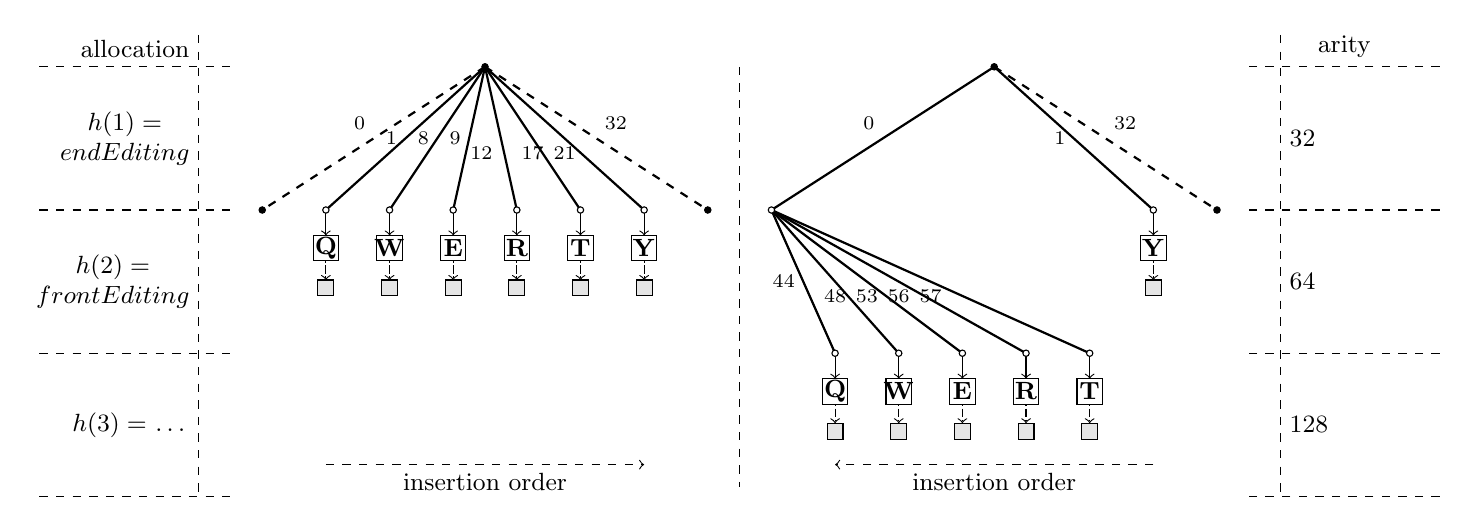
\begin{tikzpicture}[scale=1.15]

\newcommand\Y{-45}
\newcommand\ADDY{-8}

  \small
  \draw[dashed] (0pt,10pt) -- (0pt,3*\Y pt);
  \draw[dashed] (-50pt,0 pt) -- node[anchor=south]{allocation} (10pt,0 pt);
  \draw[dashed] (-50pt,\Y pt) -- (10pt,\Y pt);
  \draw[dashed] (-50pt,2*\Y pt) -- (10pt,2*\Y pt);
  \draw[dashed] (-50pt,3*\Y pt) -- (10pt,3*\Y pt);

  \draw (0pt,0.5*\Y pt)
  node[anchor=east, align=center]{$h(1) =$\\$endEditing$};
  \draw (0pt,1.5*\Y pt)
  node[anchor=east, align=center]{$h(2) =$\\$frontEditing$};
  \draw (0pt,2.5*\Y pt)
  node[anchor=east]{$h(3) =$ \ldots};

  \small
  \draw[dashed] (340pt,10pt) -- (340pt,3*\Y pt);
  \draw[dashed] (390pt,0 pt) --node[anchor=south]{arity}(330pt,0 pt);
  \draw[dashed] (390pt,\Y pt) -- (330pt,\Y pt);
  \draw[dashed] (390pt,2*\Y pt) -- (330pt,2*\Y pt);
  \draw[dashed] (390pt,3*\Y pt) -- (330pt,3*\Y pt);

  \draw (340pt,0.5*\Y pt)
  node[anchor=west, align=center]{$32$};
  \draw (340pt,1.5*\Y pt)
  node[anchor=west, align=center]{$64$};
  \draw (340pt,2.5*\Y pt)
  node[anchor=west, align=center]{$128$};

  \begin{scope}[shift={(90pt,0pt)}]
  \draw[->,dashed](-50pt,3*\Y + 10 pt) -- node[anchor=north]{insertion order}
  (50pt, 3*\Y + 10 pt);

  %% node to node
  \scriptsize
  \draw[dashed, thick] (0pt,0pt) -- node[anchor=south east]{0} (-70pt,\Y pt);
  \draw[thick] (0pt,0pt) -- node[anchor=east]{1} (-50pt,\Y pt);
  \draw[thick] (0pt,0pt) -- node[anchor=east]{8} (-30pt,\Y pt);
  \draw[thick] (0pt,0pt) -- node[anchor=east]{9} (-10pt,\Y pt);
  \draw[thick] (0pt,0pt) -- node[anchor=north east]{12} ( 10pt,\Y pt);
  \draw[thick] (0pt,0pt) -- node[anchor=north]{17} ( 30pt,\Y pt);
  \draw[thick] (0pt,0pt) -- node[anchor=north]{21} ( 50pt,\Y pt);
  \draw[dashed, thick] (0pt,0pt) -- node[anchor=south west]{32} ( 70pt,\Y pt);
  \small
  %% node to element
  \draw[->] (-50pt,\Y pt) -- (-50pt,\ADDY + \Y pt);
  \draw[->] (-30pt,\Y pt) -- (-30pt,\ADDY + \Y pt);
  \draw[->] (-10pt,\Y pt) -- (-10pt,\ADDY + \Y pt);
  \draw[->] ( 10pt,\Y pt) -- ( 10pt,\ADDY + \Y pt);
  \draw[->] ( 30pt,\Y pt) -- ( 30pt,\ADDY + \Y pt);
  \draw[->] ( 50pt,\Y pt) -- ( 50pt,\ADDY + \Y pt);

  %% element to desambiguator
  \draw[->,densely dashdotted] ( -50pt,\ADDY + \Y pt) --
  ( -50pt,2.75*\ADDY + \Y pt);
  \draw[->,densely dashdotted] ( -30pt,\ADDY + \Y pt) --
  ( -30pt,2.75*\ADDY + \Y pt);
  \draw[->,densely dashdotted] ( -10pt,\ADDY + \Y pt) --
  ( -10pt,2.75*\ADDY + \Y pt);
  \draw[->,densely dashdotted] (  10pt,\ADDY + \Y pt) --
  (  10pt,2.75*\ADDY + \Y pt);
  \draw[->,densely dashdotted] (  30pt,\ADDY + \Y pt) --
  (  30pt,2.75*\ADDY + \Y pt);
  \draw[->,densely dashdotted] (  50pt,\ADDY + \Y pt) --
  (  50pt,2.75*\ADDY + \Y pt);

  \draw[fill=black] (  0pt,  0pt) circle (1pt);
  \draw[fill=black] (-70pt,\Y pt) circle (1pt);
  \draw[fill=white] (-50pt,\Y pt) circle (1pt);
  \draw[fill=white] (-30pt,\Y pt) circle (1pt);
  \draw[fill=white] (-10pt,\Y pt) circle (1pt);
  \draw[fill=white] ( 10pt,\Y pt) circle (1pt);
  \draw[fill=white] ( 30pt,\Y pt) circle (1pt);
  \draw[fill=white] ( 50pt,\Y pt) circle (1pt);
  \draw[fill=black] ( 70pt,\Y pt) circle (1pt);

  %% elements
  \draw[fill=white](-50pt,-4 + \ADDY + \Y pt)
  node{\textbf{Q}}+(-4pt,-4pt)rectangle+(4pt,4pt) ;
  \draw[fill=white](50pt,-4 + \ADDY + \Y pt)
  node{\textbf{Y}} +(-4pt,-4pt) rectangle +(4pt,4pt) ;
  \draw[fill=white]( 10pt,-4 + \ADDY + \Y pt)
  node{\textbf{R}} +(-4pt,-4pt) rectangle +(4pt,4pt) ;
  \draw[fill=white] ( -30pt,-4 + \ADDY + \Y pt)
  node{\textbf{W}} +(-4pt,-4pt) rectangle +(4pt,4pt) ;
  \draw[fill=white] ( -10pt,-4 + \ADDY + \Y pt)
  node{\textbf{E}} +(-4pt,-4pt) rectangle +(4pt,4pt) ;
  \draw[fill=white]( 30pt,-4 + \ADDY + \Y pt)
  node{\textbf{T}} +(-4pt,-4pt) rectangle +(4pt,4pt) ;

  %% desambiguator
  \draw[fill=gray!20] (-50pt,-2.5 + 2.75 * \ADDY + \Y pt)
  +(-2.5pt,-2.5pt) rectangle +(2.5pt,2.5pt);
  \draw[fill=gray!20] (-30pt,-2.5 + 2.75 * \ADDY + \Y pt)
  +(-2.5pt,-2.5pt) rectangle +(2.5pt,2.5pt);
  \draw[fill=gray!20] (-10pt,-2.5 + 2.75 * \ADDY + \Y pt)
  +(-2.5pt,-2.5pt) rectangle +(2.5pt,2.5pt);
  \draw[fill=gray!20] ( 10pt,-2.5 + 2.75 * \ADDY + \Y pt)
  +(-2.5pt,-2.5pt) rectangle +(2.5pt,2.5pt);
  \draw[fill=gray!20] ( 30pt,-2.5 + 2.75 * \ADDY + \Y pt)
  +(-2.5pt,-2.5pt) rectangle +(2.5pt,2.5pt);
  \draw[fill=gray!20] ( 50pt,-2.5 + 2.75 * \ADDY + \Y pt)
  +(-2.5pt,-2.5pt) rectangle +(2.5pt,2.5pt);

%%%%%%%%%%%%%%%%%%%%%%%%%%%%%%%%%%%%%%%%%%%%%%%%%%%%%%%%%%%%%%%%%%%%%%

  \draw[dashed] (80pt,0pt) -- (80pt,-132pt);

\begin{scope}[shift={(160pt,0pt)}]
  \draw[->,dashed](50pt,3*\Y + 10 pt)--node[anchor=north]{insertion order}
  (-50pt,3*\Y + 10 pt);
  %% node to node
  \scriptsize
  \draw[thick] (0pt,0pt) -- node[anchor=south east]{0} (-70pt,\Y pt);
  \draw[thick] (0pt,0pt) -- node[anchor=east]{1} (50pt, \Y pt); %% Y
  \draw[thick] (-70pt, \Y pt) -- node[anchor=north]{57} (30pt, 2 * \Y pt); %% T
  \draw[thick] (-70pt, \Y pt) -- node[anchor=north]{56} (10pt, 2 * \Y pt); %% R
  \draw[thick] (-70pt, \Y pt) -- node[anchor=north]{53}(-10pt, 2 * \Y pt);%% E
  \draw[thick] (-70pt, \Y pt) -- node[anchor=north]{48}(-30pt,2 * \Y pt); %% W
  \draw[thick] (-70pt, \Y pt) -- node[anchor=east]{44}(-50pt,2 * \Y pt); %% Q
  \draw[dashed, thick] (0pt,0pt) -- node[anchor=south west]{32} (70pt,\Y pt);
  \small

  %% node to element
  \draw[->] ( 50pt, \Y pt) -- ( 50pt, \ADDY + \Y pt); %% Y
  \draw[->] ( 30pt, 2* \Y pt) -- ( 30pt, \ADDY + 2 *\Y pt); %% T
  \draw[->] ( 10pt, 2 *\Y pt) -- ( 10pt, \ADDY + 2 *\Y pt); %% R
  \draw[->] (-10pt, 2 *\Y pt) -- (-10pt, \ADDY + 2 *\Y pt); %% E
  \draw[->] (-30pt, 2 *\Y pt) -- (-30pt, \ADDY + 2 *\Y pt); %% W
  \draw[->] (-50pt, 2 *\Y pt) -- (-50pt, \ADDY + 2 *\Y pt); %% Q

  %% element to desambiguator
  \draw[->,densely dashdotted]
  ( 50pt, \ADDY + \Y pt) -- ( 50pt,2.75*\ADDY+\Y pt); %% Y
  \draw[->,densely dashdotted]
  ( 30pt, \ADDY + 2* \Y pt) -- ( 30pt,2.75*\ADDY+ 2* \Y pt); %% T
  \draw[->,densely dashdotted]
  ( 10pt, \ADDY + 2* \Y pt) -- ( 10pt,2.75*\ADDY+ 2* \Y pt); %% R
  \draw[->,densely dashdotted]
  ( -10pt, \ADDY + 2 *\Y pt) -- (-10pt,2.75*\ADDY+ 2* \Y pt); %% E
  \draw[->,densely dashdotted]
  ( -30pt, \ADDY + 2 *\Y pt) -- (-30pt,2.75*\ADDY+ 2*\Y pt); %% W
  \draw[->,densely dashdotted]
  ( -50pt, \ADDY + 2* \Y pt) -- (-50pt,2.75*\ADDY+ 2*\Y pt); %% Q

  %% node
  \draw[fill=black] (0pt,0pt) circle (1pt); %% rooot
  \draw[fill=white] ( 50pt, \Y pt) circle (1pt); %% Y
  \draw[fill=white] (-70pt, \Y pt) circle (1pt); %% 0
  \draw[fill=white] ( 30 pt, 2 * \Y pt) circle (1pt); %% T
  \draw[fill=white] ( 10 pt, 2 * \Y pt) circle (1pt); %% R
  \draw[fill=white] (-10 pt, 2 * \Y pt) circle (1pt); %% E
  \draw[fill=white] (-30 pt, 2 * \Y pt) circle (1pt); %% W
  \draw[fill=white] (-50 pt, 2 * \Y pt) circle (1pt); %% Q
  \draw[fill=black] ( 70pt, \Y pt) circle (1pt);


  %% elements
  \draw[fill=white] ( 50pt, -4 + \ADDY + \Y pt)
  node{\textbf{Y}} +(-4pt,-4pt) rectangle +(4pt,4pt) ; %% Y
  \draw[fill=white] ( 30pt, -4 + \ADDY +  2 *\Y pt)
  node{\textbf{T}} +(-4pt,-4pt) rectangle +(4pt,4pt) ; %% T
  \draw[fill=white] ( 10pt, -4 + \ADDY +  2* \Y pt)
  node{\textbf{R}} +(-4pt,-4pt) rectangle +(4pt,4pt) ; %% R
  \draw[fill=white] (-10pt, -4 + \ADDY + 2 *\Y pt)
  node{\textbf{E}} +(-4pt,-4pt) rectangle +(4pt,4pt) ; %% E
  \draw[fill=white] (-30pt, -4 + \ADDY + 2 * \Y pt)
  node{\textbf{W}} +(-4pt,-4pt) rectangle +(4pt,4pt) ; %% W
  \draw[fill=white] (-50pt, -4 + \ADDY + 2 *\Y pt)
  node{\textbf{Q}} +(-4pt,-4pt) rectangle +(4pt,4pt) ; %% Q

  %% desambiguator
  \draw[fill=gray!20]( 50pt, -2.5 + 2.75 * \ADDY + \Y pt)
  +(-2.5pt,-2.5pt) rectangle +(2.5pt,2.5pt);
  \draw[fill=gray!20]( 30pt, -2.5 + 2.75 * \ADDY +2 *\Y pt)
  +(-2.5pt,-2.5pt) rectangle +(2.5pt,2.5pt);
  \draw[fill=gray!20]( 10pt, -2.5 + 2.75 * \ADDY +2*\Y pt)
  +(-2.5pt,-2.5pt) rectangle +(2.5pt,2.5pt);
  \draw[fill=gray!20](-10pt, -2.5 + 2.75 * \ADDY +2*\Y pt )
  +(-2.5pt,-2.5pt) rectangle +(2.5pt,2.5pt);
  \draw[fill=gray!20](-30pt, -2.5 + 2.75 * \ADDY +2*\Y pt)
  +(-2.5pt,-2.5pt) rectangle +(2.5pt,2.5pt);
  \draw[fill=gray!20](-50pt, -2.5 + 2.75 * \ADDY +2*\Y pt) 
  +(-2.5pt,-2.5pt) rectangle +(2.5pt,2.5pt);

\end{scope}
\end{scope}

\end{tikzpicture}

  \caption{\label{fig:lseqtreeexample} Example of \NAME{}'s exponential trees
    with two antagonist editing behaviours to create the sequence of characters
    $QWERTY$. Thanks to its hash function, \NAME{} transfers the allocation of
    paths to the sub-allocation functions designed for front-editing and
    end-editing at first and second level respectively for this
    example. Furthermore, the arity is doubled at each level of the
    tree. Contrarily to the example given in Figure~\ref{fig:allocpathexample},
    the trees do not grow linearly.}
\end{figure*}

\begin{asparadesc}
\item[Example:] Similarly to the example of Figure~\ref{fig:allocpathexample})
  the example given in Figure~\ref{fig:lseqtreeexample} depicts the resulting
  trees after two antagonist scenarios creating the sequence
  $QWERTY$ \begin{inparaenum}[(i)] \item the left-to-right editing sequence
    [($Q,\,0$), ($W,\,1$), \ldots] and \item the right-to-left editing sequence
    [($Y,\,0$), ($T,\,0$), \ldots]. \end{inparaenum} In both cases, the
  exponential tree of \NAME{} starts with an arity $32$ and doubles it at each
  level. Also, it uses the $frontEditing$ and $endEditing$ sub-allocation
  functions at the first and the second level of the tree respectively. Since
  the first level of the tree uses the function $endEditing$, the scenario
  involving the left-to-right editing sequence results in a tree of depth 1. On
  the other hand, contrarily to the allocation function presented in
  Figure\ref{fig:allocpathexample}), the antagonist scenario does not increase
  very much the depth of the tree. Indeed, the identifiers of \NAME{} quickly
  reach a level of the tree where the sub-allocation function is designed to
  handle the right-to-left editing behaviour.
\end{asparadesc}

\begin{asparadesc}
\item [The function allocDis] creates the di\-sam\-bi\-gua\-tors which have two
  goals.  It ensures the uniqueness of the triples, even in presence of
  concurrency and it guarantees that triples can always be inserted between two
  other triples even when the paths of the latter are identical. The example of
  Figure~\ref{fig:allocpathexample} illustrates the need of comparisons that
  preserve the order given by the paths and also examines the
  disambiguators. During the editing session, the insertion between the
  elements $W$ and $T$ resulted in an identical path [$29$]. Therefore, without
  $allocDis$, the order among $W$ and $T$ is ambiguous, and inserting between
  them becomes impossible. Indeed, if any path [$29.X$] is greater than [$29$],
  the newly inserted elements will always end up after the $W$ and $T$ in the
  sequence. Consequently, the disambiguators are necessary to build an
  allocation function for sequences.
\end{asparadesc}

A disambiguator is a list of pairs $\langle source,\, clock\rangle$. Similarly
to the tree of paths, the set of all disambiguators can be represented as a
tree equipped with a lexicographic total order
$(\mathcal{D},\, <_{\mathcal{D}})$. While the total order $<_{\mathcal{P}}$
ultimately compares two numbers, the total order $<_{\mathcal{D}}$ compares two
pairs. With the same notation than $allocPath$, let $\langle s_1,\, c_1\rangle$
and $\langle s_2,\,c_2\rangle$ be the $l+1$ couples of the disambiguators $d_j$
and $d_k$ respectively. $d_j <_{\mathcal{D}}d_k$ iff $s_1 < s_2$, or if
$s_1=s_2$, $c_1 < c_2$.

\begin{algorithm}
  
\small
\algrenewcommand{\algorithmiccomment}[1]{\hskip2em$\rhd$ #1}
\newcommand*{\comment}[1]{$\rhd$ #1}

\newcommand{\LINEIFTHEN}[2]{%
  \algorithmicif\ {#1}\ \algorithmicthen\ {#2} %
  }

  \begin{algorithmic}[1]
    \State \textbf{let} $site$ \hfill \comment{the unique site identifier}
    \State \textbf{let} $counter \leftarrow 0$ \hfill \comment{a local counter}
    \Statex
    \Function{allocDis}{$p \in \mathcal{I},\, path\in\mathcal{P},\, q \in
      \mathcal{I}$} $\rightarrow \mathcal{D}$
    \State \textbf{let} $dis \leftarrow [\,]$;
    \State $counter \leftarrow counter + 1$;
    \For{$i$ \textbf{from} $1$ \textbf{to} $|path|$}
    \State $dis[i] \leftarrow \langle site,\, counter \rangle$;
    \State \LINEIFTHEN {$path[i]=q.P[i]$} {$dis[i] \leftarrow q.D[i];$}
    \State \LINEIFTHEN {$path[i]=p.P[i]$} {$dis[i] \leftarrow p.D[i];$}
    \EndFor
    \State \textbf{return} $dis$;
    \EndFunction
  \end{algorithmic}

  \caption{\label{algo:allocdis}The function $allocDis$ of \NAME{}}
\end{algorithm}

Algorithm~\ref{algo:allocdis} describes the allocation of a disambiguator which
preserves the intention of the peer that performed the insertion. Identically
to Lamport timestamps, it uses a unique site identifier and a monotonically
increasing counter. Basically, it copies the disambiguator of its neighbours at
the depth where they are equal, and, if none is equal, it copies its own site
and counter. The latter case happens at least once per insertion which
guarantees the uniqueness of each identifier. The space complexity of
disambiguator is upper-bounded by the length of the new path. Furthermore,
depending on the scenario, it can be drastically compressed.

Let us go back to the example in Figure~\ref{fig:treemodelexample}. In this
tree, collaborator $p_1$ inserts the character $R$ between the two pairs
$\langle [3],\, E\rangle$ and $\langle [4],\, T\rangle$. The resulting path is
$[3.1]$. Now, we add the disambiguators $\delta_E = [\langle 2,\,1\rangle]$
meaning that it is the first insertion of collaborator $p_2$, and
$\delta_T = [\langle 3,\,1\rangle]$ meaning that it is the first insertion of
collaborator $p_3$. The resulting path associated with $R$ is $[3.1]$. Since
the first integer of the path of $R$ is similar to the path of the character
$E$, the algorithm copies the first part of $\delta_E$. Then, since none of the
adjacent pairs have a length of $2$, the algorithm copies the values of $p_1$,
i.e. $\langle 1,\,1\rangle$. The resulting disambiguator is
$[\langle 2,\,1\rangle,\, \langle 1,\,1\rangle]$. This way, $p_1$ inserts a new
character between $E$ and $R$. As we get the path $[3.0.X]$, the resulting
disambiguator is
$[\langle 2,\,1\rangle,\,\langle 1,\,2\rangle,\,\langle 1,\,2\rangle]$.

\begin{asparadesc}
\item [The global total order] $(\mathcal{I}, <_{\mathcal{I}})$ is a
  composition of the aforementioned sets $\mathcal{P}$ and $\mathcal{D}$, and
  their respective total orders $(\mathcal{P},\, <_{\mathcal{P}})$ and
  $(\mathcal{D},\, <_{\mathcal{D}})$.
\end{asparadesc}

The global total order is defined as:
$\forall p,\,q \in \mathcal{I}, p<q \Leftrightarrow \exists i$ with
$\forall_{k=0}^{i-1}, \, p.P(k) = q.P(k) \wedge p.D(k) = q.D(k)$ such that
$\exists j=i+1$ with
$p.P(j) < q.P(j) \vee (p.P(j) = q.P(j) \wedge p.D(j) < q.D(j))$.

\subsection{Space complexity}
\label{sec:spacecomplexity}

In text editing, most of the editing behaviours can be empirically summarised
as a composition of two basic editing behaviours.
\begin{inparaenum}[(i)]
\item The random editing behaviour where the author inserts new elements at
  what appears random positions in the sequence. For instance, this behaviour
  mostly arises when syntactic corrections are performed, e.g., the author
  writes $QWETY$ and realises that the $R$ is missing. She adds the missing
  character in a second time.
\item The monotonic editing behaviour where the author repeatedly inserts new
  elements between the last inserted element and an adjacent element (after or
  before exclusively). For instance, when an author writes $QWERTY$, she
  generally starts from the first letter $Q$ to the last letter of the word
  $Y$. On the opposite, insertions in a logfile are usually performed at the
  beginning for practical reasons.
\end{inparaenum}

As a consequence, we focus on the space complexity analysis of \NAME{} to
random and monotonic editing behaviours to which we add a worst-case complexity
analysis.  The analysis does not include an average case since it requires to
know the average distribution of the position of edits performed by a human
collaborator which is obviously very complex.

Also, since the space complexity of disambiguators provided by $allocDis$ is
upper bounded by the paths allocated by $allocPath$, the space complexity
analysis of the path is reduced to the space complexity of the identifiers of
\NAME{}.

\begin{asparadesc}
\item [Random editing behaviour] is equivalent to a uniform distribution of the
  positions of the insert operations within the range of the sequence. As a
  consequence, the underlying tree of the allocation function is
  balanced. Depending on the depth $k$, the tree can hold a number $n$ of
  elements: \begin{equation} n = \sum\limits_{i=0}^{k}
    {2^{(i^2-i)/2}} \end{equation} Therefore, after $n$ insert operations
  performed on the sequence, the number of concatenations composing a path is
  upper-bounded by:
  \begin{equation} O(\sqrt{log\,n}) \end{equation} Furthermore, a path is a
  sequence of numbers $[a_1.a_2\ldots$ $a_k]$. Each number $a_j$ requires one
  more bit than its preceding number $a_{j-1}$. Let $b$ be the number of bits
  to encode $a_0$. Thus, a path is encoded by:
  \begin{equation} \sum\limits_{i=1}^{k}b+i = kb + k(k+1)/2 = O(k^2) \,
    bits \end{equation} By a simple replacement of $k$ in the latter expression
  by the former, the resulting space complexity of identifiers is the optimal
  bound:
  \begin{equation} O(log\,n) \, bits \end{equation}
  
\item[Monotonic editing behaviour] is similar to repeatedly:
  \begin{inparaenum}[(i)]
  \item fill one branch of the tree and
  \item increase the depth of the tree.
  \end{inparaenum} Consequently, with a classical K-ary tree, the number of
  concatenations of the paths grows linearly. However, using an
  exponential tree, the number of available nodes in a branch still grows
  exponentially. Depending on the depth $k$, the tree can hold $n$ elements:
  \begin{equation} n = 2^{k+1}-1 \end{equation} Therefore, the number of
  concatenations of the path is:
  \begin{equation} O(log\,n) \end{equation} After the replacement of the
  variable $k$, we obtain the following space complexity of the monotonic
  editing behaviour:
  \begin{equation} O((log\,n)^2) \, bits \end{equation}

\item [The worst-case] corresponds to one element per level in the
  tree. Therefore, the growth of the paths is linear for both K-ary tree and
  exponential tree. Thus, when $n$ insert operations are performed on the
  sequence, the number of concatenations composing a path is:
  \begin{equation} O(n) \end{equation} However, while the space complexity
  remains linear in the case of the N-ary tree, the exponential tree implies
  the following space complexity on its identifiers:
  \begin{equation} O(n^2) \, bits \end{equation}
\end{asparadesc}

\begin{table}
  \centering
  \begin{tabular}{@{}lccc@{}}
    \toprule
    & Random & Monotonic & Worst \\ \cmidrule{2-4}
    Id.size & $O(\sqrt{log\,n})$ & $O(log\,n)$ & $O(n)$ \\ \midrule
    Id.bit-length & \multicolumn{3}{c}{ $\sum\limits_{i=1}^{k}b+i =
      kb + k(k+1)/2 = O(k^2)$} \\ \midrule
    Space complexity & $O(log\,n)$ & $O((log\,n)^2)$ &
    $O(n^2)$ \\ \bottomrule
  \end{tabular}
  \caption{Spatial complexity of \NAME{}. Where $n$ is the number
    of insert operations performed. $k$ is the size of an identifier, i.e.,
    the number of concatenations. And $b$ the starting bit-length of numbers
    composing the identifiers.}
\end{table}

To summarise, the space complexity analysis reveals that the allocation
function \NAME{} sacrifices on the worst-case space complexity to improve the
space complexity of the monotonic editing behaviours. Nevertheless, in text
editing, the worst-case happens with a very low probability compared the other
cases. Furthermore, it is worth noting that usually, the authors do not write a
document in a single round, starting from the beginning to go straight up to
the end (as the monotonic analysis could suggest). On the contrary, the authors
write sections, structure the documents, perform corrections, rewrite parts of
the document, reorganise, etc. This behaviour (between random and monotonic
behaviour) tends to even up the branches of the underlying tree of \NAME{}. In
the case of random editing, the space complexity is asymptotically optimal
$O(log\,n)$ while it is very interesting in a "normal setting" $O((log\,n)^2)$.

%%% Local Variables: 
%%% mode: latex
%%% TeX-master: "../paper"
%%% End: 

% LocalWords:  disambiguator neighbours
